\section{Présentation de Python}

Python est un langage de programmation inventé par Guido van Rossum en 1990. Son nom est une référence à la série télévisée Monty Python, dont van Rossum était fan.

Au fil des années, le langage a évolué. En 2000, on voit apparaître \texttt{Python 2.0}, et en 2008, \texttt{Python 3.0}.
Actuellement, deux version de Python coexistent : \texttt{Python 2.7}, et \texttt{Python 3.6}. Nous utiliserons dans ce cours la dernière version.

Python est un langage très utilisé. Sa syntaxe simple en fait un des langages les plus appréciés pour écrire des \textit{scripts}. Il est aussi utilisé dans le monde scientifique, dans des domaines tels que la science des données et l'intelligence artificielle.

Dans ce cours, on utilisera le Python pour écrire des programmes, qu'on pourra exécuter sur un Raspberry Pi.

\section{Qu'est-ce qu'un programme?}
Les ordinateurs sont des outils très puissants, pour peu qu'on arrive à leur communiquer ce qu'on aimerait obtenir. On entend souvent dire qu'un ordinateur ne comprend qu'un langage très basique : le langage binaire, une suite de 0 et de 1. Du point de vue des microprocesseurs, on peut voir ça ainsi : soit le courant passe, soit il ne passe pas. En combinant ces deux états d'une manière bien précise, on peut effectuer des calculs.

Cependant, écrire un quelconque programme directement en binaire, c'est quasiment mission impossible, même pour un programme très basique. Il faut passer par une étape de traduction, et c'est ici que ça devient intéressant! L'idée générale est d'écrire du code dans un langage de programmation, et de le transformer en langage machine/binaire.

Il y a deux manières de traduire du code.
\begin{itemize}
    \item \emph{La compilation :} On convertit immédiatement le code en langage machine. L'avantage, c'est que l'ordinateur comprend directement. Par contre, il faudra recommencer cette étape pour chaque système d'exploitation différents (Windows, macOS, Linux, ...).
    \item \emph{L'interprétation :} on va ici passer par un intermédiaire : \textit{l'interpréteur}. C'est un programme qui lit et traduit le code en temps réel. C'est un processus plus lent, mais qui offre un grand avantage : on ne doit plus faire plusieurs versions pour chaque système d'exploitation, puisque c'est l'interpréteur qui se charge de la traduction! On dit d'un tel langage qu'il est \textit{multi-plateformes}.
\end{itemize}

%%% Au cours, on peut donner un exemple : compilation = traduire un texte en chinois et en arabe. Interprétation = le donner à un mec qui sait parler chinois et arabe. On doit pas traduire nous-même mais ça prend plus de temps.

Il existe une autre manière de classer les langages de programmation. Au plus ils ressemblent à du langage machine, au plus ils sont \textit{bas niveau}. Au contraire, au plus un langage de programmation se rapproche du langage humain, au plus il est \textit{haut-niveau}.

Le Python est un langage interprété, et haut-niveau, ce qui en fait un excellent choix pour débuter en programmation : on peut l'exécuter aisément sur de nombreux systèmes d'exploitation, et le code est assez lisible. Mais il ne faut pas s'y tromper : ce n'est pas parce qu'il est haut-niveau qu'il n'est pas puissant, bien au contraire! 

\section{Environnement de développement}
Le Python est interprété, il nous faut donc un interpréteur! Il s'agit simplement d'un programme qui va lire notre code, et exécuter en temps réel les instructions qu'on lui donne.

Théoriquement, c'est le seul outil dont on a réellement besoin. Pratiquement, un développeur s'entoure d'une suite logicielle qui lui rend la vie bien plus facile. On utilisera énormément un \textit{éditeur de code}. C'est un éditeur de texte, à la manière de Microsoft Word, mais spécialisé dans un ou plusieurs langages de programmation. Il va notamment permettre de colorer le code pour le lire plus facilement, indenter automatiquement les lignes, les numéroter, etc.

\subsection{lancer un programme python}

On peut tout-à-fait utiliser l'éditeur de code et l'interpréteur séparément. Pour ce faire, il faut d'abord créer un fichier texte.\\
par exemple, ajoutons un nouveau fichier \textit{helloworld.txt} sur le bureau, qui contient exactement:
\begin{python}
print("Hello world !")
\end{python}
(notez que contrairement à Windows, l'extension .txt n'est pas nécéssaire à Raspbian, le système d'exploitation utilisé ici sur les raspberry pi.)
\\
Voilà notre premier programme en Python! Il sera expliqué par la suite, mais d'abord, lançons-le avec une invite de commande, aussi nommée le terminal. il se trouve dans la liste des programmes installés, ou en cliquant directement sur son icone noir dans la barre des tâches, ou encore avec le raccourci clavier $Ctrl + Alt + t$, mais le plus simple est de l'ouvrir via un click-droit sur le bureau->ouvrir en ligne de commande.

\subsection{Installer Spyder}

Les instructions suivantes permettent d'installer l'IDE \textit{Spyder}.

\begin{enumerate}
    \item Se rendre sur \url{https://www.continuum.io/downloads}.
    \item Télécharger l'installateur et suivre les instructions d'installation de celui-ci.
    \item Une fois l'installation terminée, lancer le programme \textit{Anaconda Navigator}.
    \item Depuis l'écran qui apparaît, lancer \textit{Spyder}.
\end{enumerate}

\subsection{Présentation de l'interface}

\begin{figure}[h!]
\begin{center}
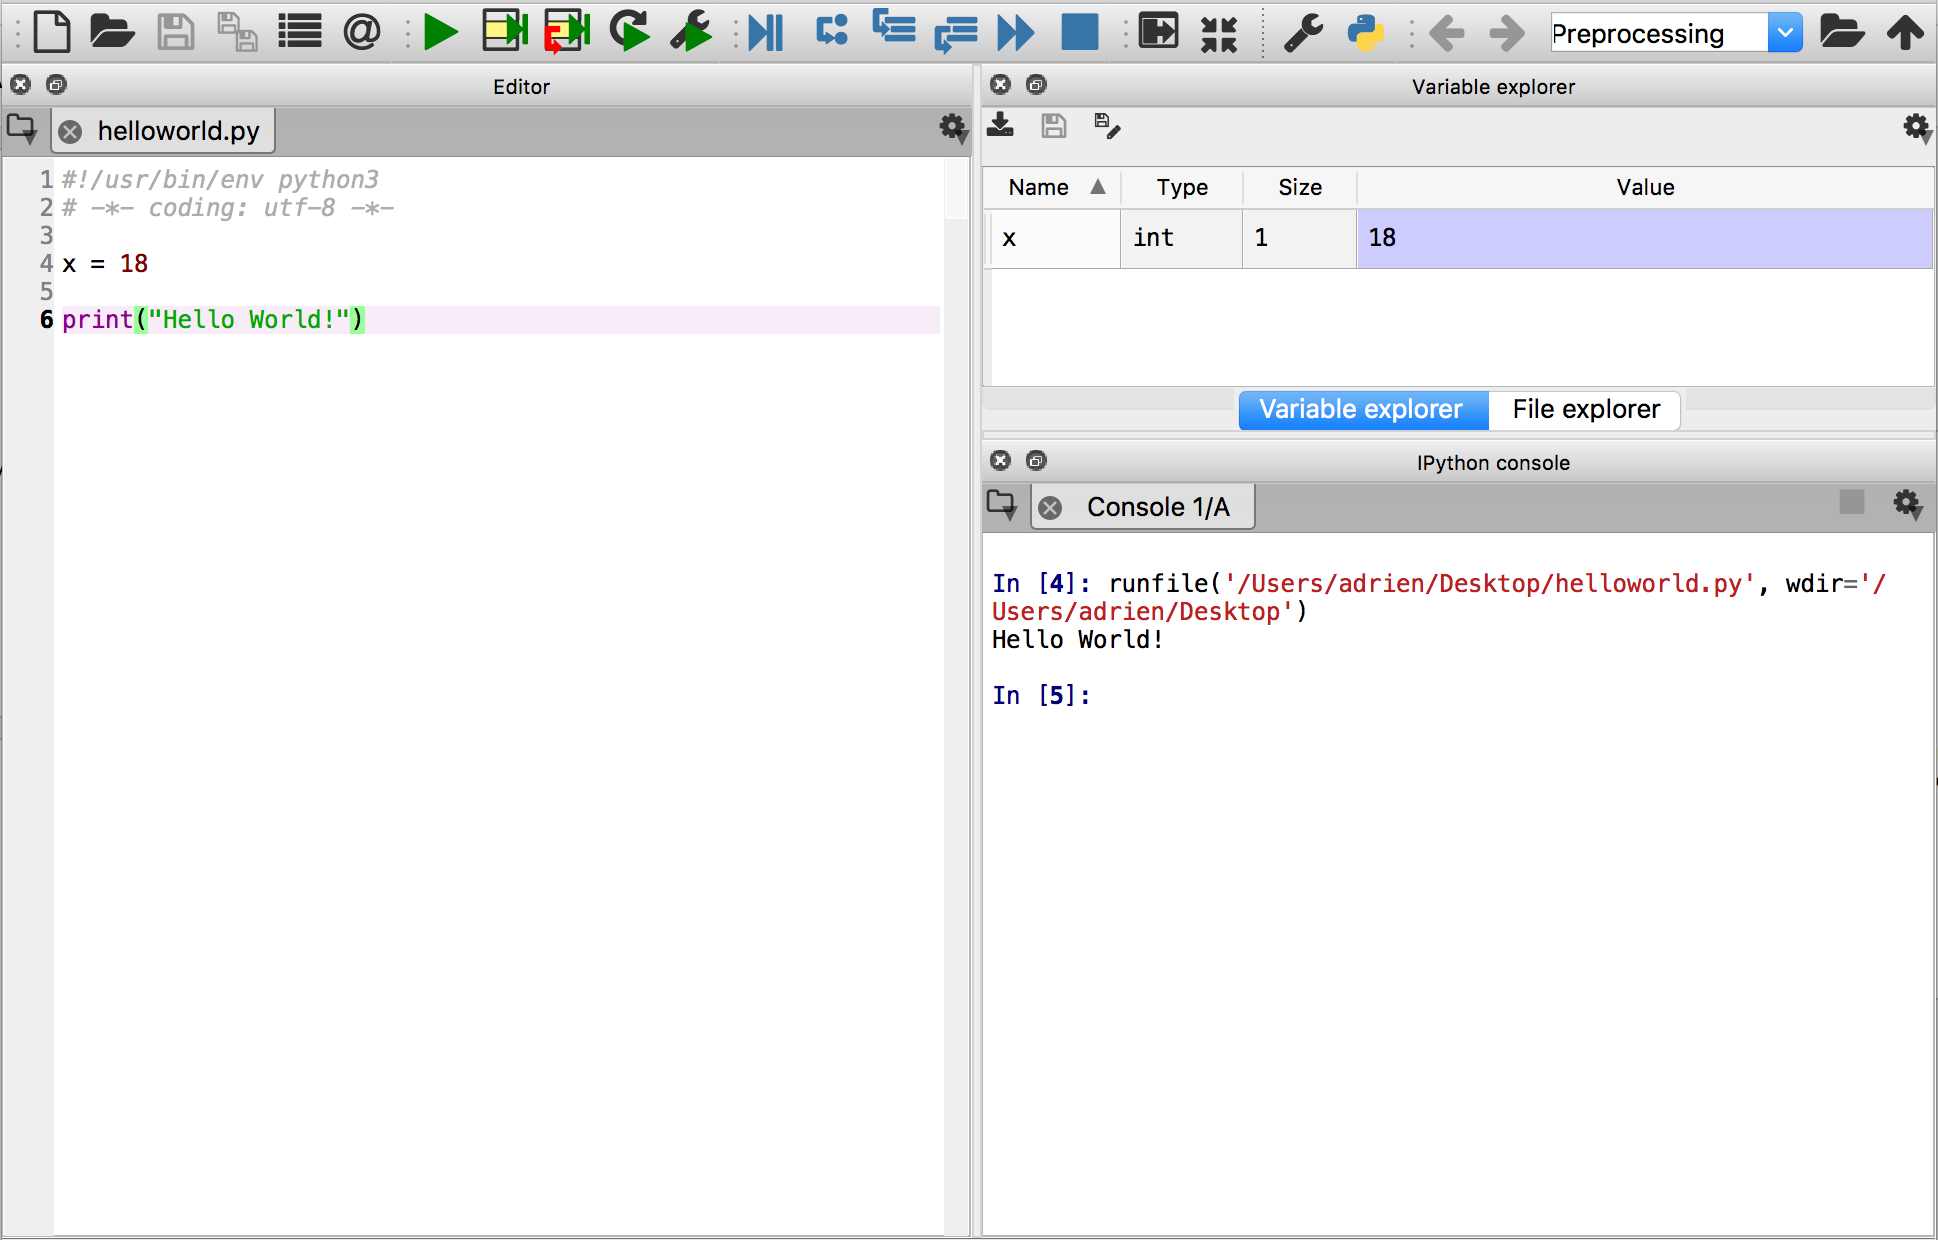
\includegraphics[width=15cm]{img/spyder.png}
\end{center}
\caption{Interface de Spyder}
\label{spyder}
\end{figure}

L'interface est simple à prendre en main. On retrouve 3 panneaux que nous utiliserons.
\begin{enumerate}
    \item A gauche, l'éditeur de code. C'est ici que nous écrirons le code source.
    \item En haut à droite, l'explorateur de variables. Probablement plus utile au début de l'apprentissage, on peut y voir les variables déclarées, et leur type.
    \item En bas à droit, la console. C'est ici que s'afficheront les résultats de nos programmes. On peut aussi directement y taper du code.
\end{enumerate}

Tout en haut, on trouve la barre d'outils. Les trois boutons de gauche servent respectivement à créer un fichier, ouvrir un fichier, et sauver le fichier. Enfin, la flèche verte permet d'exécuter le programme. Concrètement, l'interpréteur Python sera lancé, il lira le contenu de l'éditeur de code, et affichera le résultat dans la console.

\section{Premier programme}
Pour vérifier que l'installation s'est déroulée correctement et que vous disposez de tous les outils nécessaires, écrivons donc un premier programme!

Ouvrez Spyder, et créez un nouveau fichier au besoin en cliquant sur le premier bouton à gauche de la barre d'outils.

Dans l'éditeur de texte, copiez-collez le bout de code suivant :

\begin{python}
print("Hello World !")
\end{python}

Ensuite, lancez l'interpréteur en cliquant sur la flèche verte. Spyder vous demandera peut-être d'enregistrer le fichier. Nous vous invitons à enregistrer tous les programmes que nous écrirons cette semaine dans un dossier distinct.

Regardez à droite dans la console : une ligne de texte s'est affichée. Vous êtes maintenant normalement prêts à démarrer l'apprentissage du Python!